\documentclass[a4paper]{article}
\usepackage{standalone}
\usepackage{import}
\usepackage[utf8]{inputenc}
\usepackage[T1]{fontenc}
% \usepackage{fourier}
\usepackage{textcomp}
\usepackage{hyperref}
\usepackage[english]{babel}
\usepackage{url}
% \usepackage{hyperref}
% \hypersetup{
%     colorlinks,
%     linkcolor={black},
%     citecolor={black},
%     urlcolor={blue!80!black}
% }
\usepackage{graphicx} \usepackage{float}
\usepackage{booktabs}
\usepackage{enumitem}
% \usepackage{parskip}
% \usepackage{parskip}
\usepackage{emptypage}
\usepackage{subcaption}
\usepackage{multicol}
\usepackage[usenames,dvipsnames]{xcolor}
\usepackage{ocgx}
% \usepackage{cmbright}


\usepackage[margin=1in]{geometry}
\usepackage{amsmath, amsfonts, mathtools, amsthm, amssymb}
\usepackage{thmtools}
\usepackage{mathrsfs}
\usepackage{cancel}
\usepackage{bm}
\newcommand\N{\ensuremath{\mathbb{N}}}
\newcommand\R{\ensuremath{\mathbb{R}}}
\newcommand\Z{\ensuremath{\mathbb{Z}}}
\renewcommand\O{\ensuremath{\emptyset}}
\newcommand\Q{\ensuremath{\mathbb{Q}}}
\newcommand\C{\ensuremath{\mathbb{C}}}
\newcommand\F{\ensuremath{\mathbb{F}}}
% \newcommand\P{\ensuremath{\mathbb{P}}}
\DeclareMathOperator{\sgn}{sgn}
\DeclareMathOperator{\diam}{diam}
\DeclareMathOperator{\LO}{LO}
\DeclareMathOperator{\UP}{UP}
\DeclareMathOperator{\card}{card}
\DeclareMathOperator{\Arg}{Arg}
\DeclareMathOperator{\Dom}{Dom}
\DeclareMathOperator{\Log}{Log}
\DeclareMathOperator{\dist}{dist}
% \DeclareMathOperator{\span}{span}
\usepackage{systeme}
\let\svlim\lim\def\lim{\svlim\limits}
\renewcommand\implies\Longrightarrow
\let\impliedby\Longleftarrow
\let\iff\Longleftrightarrow
\let\epsilon\varepsilon
\usepackage{stmaryrd} % for \lightning
\newcommand\contra{\scalebox{1.1}{$\lightning$}}
% \let\phi\varphi
\renewcommand\qedsymbol{$\blacksquare$}

% correct
\definecolor{correct}{HTML}{009900}
\newcommand\correct[2]{\ensuremath{\:}{\color{red}{#1}}\ensuremath{\to }{\color{correct}{#2}}\ensuremath{\:}}
\newcommand\green[1]{{\color{correct}{#1}}}

% horizontal rule
\newcommand\hr{
    \noindent\rule[0.5ex]{\linewidth}{0.5pt}
}

% hide parts
\newcommand\hide[1]{}

% si unitx
\usepackage{siunitx}
\sisetup{locale = FR}
% \renewcommand\vec[1]{\mathbf{#1}}
\newcommand\mat[1]{\mathbf{#1}}

% tikz
\usepackage{tikz}
\usepackage{tikz-cd}
\usetikzlibrary{intersections, angles, quotes, calc, positioning}
\usetikzlibrary{arrows.meta}
\usepackage{pgfplots}
\pgfplotsset{compat=1.13}

\tikzset{
    force/.style={thick, {Circle[length=2pt]}-stealth, shorten <=-1pt}
}

% theorems
\makeatother
\usepackage{thmtools}
\usepackage[framemethod=TikZ]{mdframed}
\mdfsetup{skipabove=1em,skipbelow=1em}

\theoremstyle{definition}

\declaretheoremstyle[
    headfont=\bfseries\sffamily\color{ForestGreen!70!black}, bodyfont=\normalfont,
    mdframed={
        linewidth=1pt,
        rightline=false, topline=false, bottomline=false,
        linecolor=ForestGreen, backgroundcolor=ForestGreen!5,
    }
]{thmgreenbox}

\declaretheoremstyle[
    headfont=\bfseries\sffamily\color{NavyBlue!70!black}, bodyfont=\normalfont,
    mdframed={
        linewidth=1pt,
        rightline=false, topline=false, bottomline=false,
        linecolor=NavyBlue, backgroundcolor=NavyBlue!5,
    }
]{thmbluebox}

\declaretheoremstyle[
    headfont=\bfseries\sffamily\color{NavyBlue!70!black}, bodyfont=\normalfont,
    mdframed={
        linewidth=1pt,
        rightline=false, topline=false, bottomline=false,
        linecolor=NavyBlue
    }
]{thmblueline}

\declaretheoremstyle[
    headfont=\bfseries\sffamily, bodyfont=\normalfont,
    numbered = no,
    mdframed={
        rightline=true, topline=true, bottomline=true,
    }
]{thmbox}

\declaretheoremstyle[
    headfont=\bfseries\sffamily, bodyfont=\normalfont,
    numbered=no,
    % mdframed={
    %     rightline=true, topline=false, bottomline=true,
    % },
    qed=\qedsymbol
]{thmproofbox}

\declaretheoremstyle[
    headfont=\bfseries\sffamily\color{NavyBlue!70!black}, bodyfont=\normalfont,
    numbered=no,
    mdframed={
        rightline=false, topline=false, bottomline=false,
        linecolor=NavyBlue, backgroundcolor=NavyBlue!1,
    },
]{thmexplanationbox}

\declaretheorem[
    style=thmbox, 
    % numberwithin = section,
    numbered = no,
    name=Definition
    ]{definition}

\declaretheorem[
    style=thmbox, 
    name=Example,
    ]{eg}

\declaretheorem[
    style=thmbox, 
    % numberwithin = section,
    name=Proposition]{prop}

\declaretheorem[
    style = thmbox,
    numbered=yes,
    name =Problem
    ]{problem}

\declaretheorem[style=thmbox, name=Theorem]{theorem}
\declaretheorem[style=thmbox, name=Lemma]{lemma}
\declaretheorem[style=thmbox, name=Corollary]{corollary}

\declaretheorem[style=thmproofbox, name=Proof]{replacementproof}

\declaretheorem[style=thmproofbox, 
                name = Solution
                ]{replacementsolution}

\renewenvironment{proof}[1][\proofname]{\vspace{-1pt}\begin{replacementproof}}{\end{replacementproof}}

\newenvironment{solution}
    {
        \vspace{-1pt}\begin{replacementsolution}
    }
    { 
            \end{replacementsolution}
    }

\declaretheorem[style=thmexplanationbox, name=Proof]{tmpexplanation}
\newenvironment{explanation}[1][]{\vspace{-10pt}\begin{tmpexplanation}}{\end{tmpexplanation}}

\declaretheorem[style=thmbox, numbered=no, name=Remark]{remark}
\declaretheorem[style=thmbox, numbered=no, name=Note]{note}

\newtheorem*{uovt}{UOVT}
\newtheorem*{notation}{Notation}
\newtheorem*{previouslyseen}{As previously seen}
% \newtheorem*{problem}{Problem}
\newtheorem*{observe}{Observe}
\newtheorem*{property}{Property}
\newtheorem*{intuition}{Intuition}

\usepackage{etoolbox}
\AtEndEnvironment{vb}{\null\hfill$\diamond$}%
\AtEndEnvironment{intermezzo}{\null\hfill$\diamond$}%
% \AtEndEnvironment{opmerking}{\null\hfill$\diamond$}%

% http://tex.stackexchange.com/questions/22119/how-can-i-change-the-spacing-before-theorems-with-amsthm
\makeatletter
% \def\thm@space@setup{%
%   \thm@preskip=\parskip \thm@postskip=0pt
% }
\newcommand{\oefening}[1]{%
    \def\@oefening{#1}%
    \subsection*{Oefening #1}
}

\newcommand{\suboefening}[1]{%
    \subsubsection*{Oefening \@oefening.#1}
}

\newcommand{\exercise}[1]{%
    \def\@exercise{#1}%
    \subsection*{Exercise #1}
}

\newcommand{\subexercise}[1]{%
    \subsubsection*{Exercise \@exercise.#1}
}


\usepackage{xifthen}

\def\testdateparts#1{\dateparts#1\relax}
\def\dateparts#1 #2 #3 #4 #5\relax{
    \marginpar{\small\textsf{\mbox{#1 #2 #3 #5}}}
}

\def\@lesson{}%
\newcommand{\lesson}[3]{
    \ifthenelse{\isempty{#3}}{%
        \def\@lesson{Lecture #1}%
    }{%
        \def\@lesson{Lecture #1: #3}%
    }%
    \subsection*{\@lesson}
    \testdateparts{#2}
}

% \renewcommand\date[1]{\marginpar{#1}}


% fancy headers
\usepackage{fancyhdr}
\pagestyle{fancy}

\makeatother

% notes
\usepackage{todonotes}
\usepackage{tcolorbox}

\tcbuselibrary{breakable}
\newenvironment{verbetering}{\begin{tcolorbox}[
    arc=0mm,
    colback=white,
    colframe=green!60!black,
    title=Opmerking,
    fonttitle=\sffamily,
    breakable
]}{\end{tcolorbox}}

\newenvironment{noot}[1]{\begin{tcolorbox}[
    arc=0mm,
    colback=white,
    colframe=white!60!black,
    title=#1,
    fonttitle=\sffamily,
    breakable
]}{\end{tcolorbox}}

% figure support
\usepackage{import}
\usepackage{xifthen}
\pdfminorversion=7
\usepackage{pdfpages}
\usepackage{transparent}
\newcommand{\incfig}[1]{%
    \def\svgwidth{\columnwidth}
    \import{./figures/}{#1.pdf_tex}
}

% %http://tex.stackexchange.com/questions/76273/multiple-pdfs-with-page-group-included-in-a-single-page-warning
\pdfsuppresswarningpagegroup=1



\title{Math 234A: Homework 1}
\author{Lance Remigio}
\begin{document}
   \maketitle 

    \section*{Problem 1}  
        \begin{enumerate}
            \item[(i)] \textbf{(Parallelogram identity)} Let \( z,w \in \C  \). Show that 
                \[  | z + w  |^{2} + | z - w  |^{2} = 2 (| z  |^{2} + | w |^{2}).  \]
                \begin{proof}
                Let \( z,w \in \C  \) with \( z = x + iy  \) and \( w = u + iv  \) with \( x,y \in \R  \) and \( u,v \in \R  \). Our goal is to show that  
                \[   | z + w  |^{2} + | z - w  |^{2} = 2 (| z  |^{2} + | w |^{2}).    \]
                Consider \( | z - w  |^{2} \) and notice that 
                \[  z - w = (x - u) + i(y - v). \]
                By definition of the modulus, we have 
                \begin{align*}
                    | z - w  |^{2} &= (z - w) \overline{z - w} \\
                                   &= ((x-u) + i(y-v))((x-u) - i(y -v)) \\
                                   &= (x - u)^{2} + (y -v)^{2} \\
                                   &= x^{2} - 2xu + u^{2} + y^{2} - 2yv + u^{2} \\
                                   &= (x^{2} + y^{2}) - 2(xu + yv) + (u^{2} + v^{2}) \\
                                   &= | z |^{2} - 2(xu + yv) + | w |^{2}.
                \end{align*}
                Note that 
                \[  z + w = (x+u) + i(y+v). \]
                \begin{align*}
                    | z + w  |^{2} &= (z + w) \overline{(z+w)}   \\
                                   &= ((x+u) + i(y+v))((x+u) - i(y+v)) \\
                                   &= (x+u)^{2} + (y +v)^{2} \\
                                   &= x^{2} + 2xu + u^{2} + y^{2} + 2yv + v^{2} \\ 
                                   &= | z |^{2} + 2(xu + yv) + | w  |^{2}.
                \end{align*}
                Adding these two moduli together gives us
                \[ | z + w  |^{2} + | z - w  |^{2} = 2 | z  |^{2} + 2 | w |^{2} = 2 (| z | ^{2} + | w |^{2})    \]
                which is our desired result.

                \end{proof}
            \item[(ii)] \textbf{(Binomial Expansion)}: Let \( z,w \in \C  \) and \( n  \) be a positive integer. Show that 
                \[  (z + w)^{n} = \sum_{ k=  0  }^{  n  } \begin{pmatrix} 
                           n \\
                           k 
                          \end{pmatrix} z^{k} w^{n-k}    \]
                          where \( \begin{pmatrix} 
                                     n \\
                                     k 
                                    \end{pmatrix}  = \frac{ n!  }{ k! (n-k)! }. \)
        \end{enumerate}
        \begin{proof}
        Let \( z,w \in \C  \). We proceed via induction on \( n \in \Z^{+}  \) to show that 
                \[  (z + w)^{n} = \sum_{ k=  0  }^{  n  } \begin{pmatrix} 
                           n \\
                           k 
                          \end{pmatrix} z^{k} w^{n-k}    \]
                          where \( \begin{pmatrix} 
                                     n \\
                                     k 
                                    \end{pmatrix}  = \frac{ n!  }{ k! (n-k)! }. \)
        Let \( n =1  \) be our base case. Then we have  
        \begin{align*}
            \sum_{ k=0  }^{ 1 } \begin{pmatrix} 
                       n \\
                       k 
                      \end{pmatrix} z^{k } w^{n-k} &= \begin{pmatrix} 
                                1 \\ 
                                0 
                                \end{pmatrix} z^{0} w + \begin{pmatrix} 
                                           1 \\
                                           1
                                          \end{pmatrix} z^{1} w^{0}  \\
                                          &= (z + w)^{1},
        \end{align*}
        which tells us that the result holds in our base case. Now, suppose the result holds for \( n  \)th case. We will show the result holds for the \( n + 1  \) case. By our induction hypothesis, we see that
        \begin{align*}
            (z+w)^{n+1} &= (z+w) (z+w)^{n} \\
                        &= (z+w) \sum_{ k=0  }^{ n } \begin{pmatrix} 
                                   n \\
                                   k 
                                  \end{pmatrix} z^{k} w^{n-k} \\
                        &=  \sum_{ k=0  }^{ n } \begin{pmatrix} 
                                   n \\ 
                                   k 
                                  \end{pmatrix} z^{k+1} w^{n-k} + w \sum_{ k=0  }^{ n } \begin{pmatrix} 
                                             n \\
                                             k 
                                            \end{pmatrix} z^{k} w^{n-k + 1}.  
        \end{align*}
        Reordering indices in the first summation by setting \( m = k +1 \), we have
        \begin{align*}
            \sum_{ k=0  }^{ n } \begin{pmatrix} 
                                   n \\ 
                                   k 
                                  \end{pmatrix} z^{k+1} w^{n-k} + w \sum_{ k=0  }^{ n } \begin{pmatrix} 
                                             n \\
                                             k 
                                            \end{pmatrix} z^{k} w^{n-k + 1} &= \sum_{ m=1  }^{ n+1 } \begin{pmatrix} 
                                                       n \\
                                                       m-1
                                                      \end{pmatrix}  z^{m} w^{(n+1) -m} \\
                                                      &+ \sum_{ k=0  }^{ n } \begin{pmatrix} 
                                                                 n \\
                                                                 k 
                                                                \end{pmatrix}  z^{k} w^{(n-k) + 1}.
        \end{align*}
       Then separating the first and last term of each summation, respectively, we have
        \begin{align*}
            (z + w)^{n+1} &=  \begin{pmatrix} 
                                               n \\
                                               n 
                                              \end{pmatrix} z^{n} w + \sum_{ m=1  }^{ n } \begin{pmatrix} 
                                                         n \\
                                                         m-1
                                                     \end{pmatrix} z^{m} w^{(n-k)+1} + \sum_{ k=1 }^{ n } \begin{pmatrix} 
                                                                n \\
                                                                k 
                                                               \end{pmatrix}  z^{k } w^{n -k  + 1}  +  \begin{pmatrix} 
                                                                n \\
                                                                0  
                                                            \end{pmatrix} w^{n+1} \\
                                                            &=  \begin{pmatrix} 
                                               n \\
                                               n 
                                               \end{pmatrix} z^{n} w + \sum_{ k=1  }^{ n } \Bigg[ \begin{pmatrix} n \\ k  \end{pmatrix} + \begin{pmatrix} n \\ k - 1  \end{pmatrix}\Bigg] z^{k } w^{(n+1)-k}  +  \begin{pmatrix} 
                                                                n \\
                                                                0  
                                                            \end{pmatrix} w^{n+1}.
        \end{align*}
        Using the fact that 
        \[  \begin{pmatrix} n \\ k  \end{pmatrix}  + \begin{pmatrix} n \\ k - 1  \end{pmatrix}  = \begin{pmatrix} n + 1 \\ k  \end{pmatrix}     \]
        and collecting the first and last terms of the summation, we see that 
        \begin{align*}
            (z+w)^{n+1} &= \begin{pmatrix} n \\ 0  \end{pmatrix} z^{0} w^{n+1} + \sum_{ k=1  }^{ n } \begin{pmatrix} n + 1 \\ k  \end{pmatrix}  z^{k } w^{(n+1)- k} + \begin{pmatrix} n \\ n  \end{pmatrix} z^{n+1} w^{0}  \\
                        &= \sum_{ k=0  }^{ n + 1   } \begin{pmatrix} n + 1 \\ k  \end{pmatrix} z^{k } w^{(n+1) - k} 
        \end{align*}
        which completes our induction argument. 
        \end{proof}
    \section*{Problem 2}  For \( z,w \in \C  \). Define \( \langle z , w \rangle = \Re(z \overline{w}) \). (If we think of \(  \C  \) as two dimensional real vector space, then \( \langle \cdot  ,  \cdot  \rangle  \) defines an inner product on \( \C  \)). 
        \begin{enumerate}
            \item[(i)] Cauchy Schwarz Inequality: 
                Show that \( | \langle z , w \rangle |^{2} \leq | z |^{2} | w |^{2} \) for all \( z,w \in \C  \).
                \begin{proof}
                    Let \( z,w \in \C  \). Using the fact that \( | \Re(z \overline{w}) |  \leq | z  |  \) and \( | z  |  = | \overline{z} |  \), we see that  
                    \begin{align*}
                        | \langle z , w \rangle |^{2} = | \Re(z \overline{w}) |^{2} &\leq | z \overline{w} |^{2}  \\
                                                                                    &= | z  |^{2} | \overline{w}  |^{2} \\
                                                                                    &= | z  |^{2} | w |^{2}.
                    \end{align*}
                    Thus, we conclude that \( | \langle z , w \rangle |^{2} \leq | z |^{2} | w |^{2} \). 
                \end{proof}
            \item[(ii)] Triangle Inequalities: Show 
                \[  | z \pm w  | \leq | z  |  + | w  | \]
                and 
                \[  | | z  |  - | w |  | \leq | z \pm w  |  \]
                for all \( z,w \in \C  \).
                \begin{proof}
                Let \( z,w \in \C  \). We will first show that \(  | z + w  | \leq | z  |  + | w |  \). First, we will show the following results:
                \[  | z + w  |^{2} = | z |^{2} + 2 | \langle z , w \rangle | + | w |^{2} \tag{1} \]
                and 
                \[  | z - w  |^{2} = | z |^{2} - 2 | \langle z , w \rangle | + | w |^{2}. \tag{2}  \]
                Let \( z = x + iy \) and \( w = u + i v  \) for \( x,y,u,v \in \R  \). Observe that   
                \[  z + w = (x+u) + i(y +v) \]
                and 
                \[  z - w = (x-u) + i(y - v). \]
                Using the definition of the modulus, we see that
                \begin{align*}
                    | z + w  |^{2} = (z+w) \overline{(z+w)} &= ((x+u) + i(y+v)) ((x+u) - i(y+v)) \\
                                                            &= (x+u)^{2} + (y +v)^{2} \\
                                                            &= x^{2} +  2xu + u^{2} + y^{2} + 2yv + v^{2} \\
                                                            &= (x^{2} + y^{2}) + 2 (xu + yv) + (y^{2} + v^{2}) \\
                                                            &= | z |^{2} + 2 \langle z , w \rangle + | w |^{2}. \tag{since \( \langle z , w \rangle = \Re(z \overline{w}) \)}
                \end{align*} 
                Similarly, we have
                \begin{align*}
                    | z - w  |^{2} = (z-w)\overline{(z-w)} &= ((x-u) + i (y - v)) ((x-u) - i (y - v)) \\
                                                           &= (x-u)^{2} + (y - v)^{2} \\
                                                           &=  x^{2} -2xu + u^{2} + y^{2} -2yv + v^{2} \\
                                                           &= x^{2} + y^{2} -2(xu + yv) + v^{2} \\
                                                           &= (x^{2}  + y^{2}) -2 \langle z , w \rangle + (v^{2} + u^{2}) \\ 
                                                           &= | z |^{2} - 2 \langle z , w \rangle + | w |^{2}.
\end{align*}
Now, let us prove that \( | z + w  | \leq | z  |  + | w |  \). Consider \( | z + w  |^{2} \). By part (a), we see that
\begin{align*}
    | z + w  |^{2} &= | z  |^{2} + 2 \langle z , w \rangle + | w |^{2} \\
                   &\leq | z |^{2} + 2 z  w + | w |^{2} \\ 
                   &\leq | z |^{2} + 2 | z | | w |  + | w |^{2} \\
                   &= (| z |  + | w | )^{2}.
\end{align*}
By taking the square root of both sides, we see that
\[  | z + w  | \leq | z  |  + | w |. \]
Using this fact, we can see that 
\[  | z - w  |  = | z + (-w) | \leq | z  |  + | -w | = |  z  |  + | w |.  \]
To show the second inequality, consider \( | z - w  |^{2} \). Then using part (a) again, we have
\begin{align*}
    | z - w  |^{2} &= | z |^{2} - 2 \langle z , w \rangle + | w  |^{2} \\
                   & \geq | z |^{2} - 2 | z | | w |  + | w |^{2} \\ 
                   &= (| z |  - | w |)^{2}. 
\end{align*}
Thus, we see that  
\[  | z - w  | \geq |  | z  |  - | w |  |.  \]
Using this fact, we can say that 
\[  | z + w  |  = | z - (-w) | \geq | | z  |  - | -w |  | = | | z  |  - | w |  |. \]
                \end{proof}
        \end{enumerate}
    \section*{Problem 3} \textbf{(Lagrange Identity)} Let \( {z}_{1}, \dots, {z}_{n}, {w}_{1}, \dots, {w}_{n} \in \C   \). Show that    
        \[  \Big| \sum_{ k=1  }^{ n } {z}_{k} {w}_{k} \Big|^{2} = \sum_{ k=1  }^{ n } | {z}_{k} |^{2} \sum_{ k=1  }^{ n } | {w}_{k } |^{2} - \sum_{ 1 \leq i < j \leq n  }^{  } | {z}_{i} \overline{{w}_{j}} - {z}_{j} \overline{{w}_{i}} |^{2}. \]
        Use this to deduce that 
        \[  \Big| \sum_{ k=1  }^{ n } {z}_{k } {w}_{k } \Big|^{2} \leq \sum_{ k=1  }^{ n } | {z}_{k} |^{2} \sum_{ k=1  }^{ n } | {w}_{k } |^{2}. \]
        \begin{proof}
        We will show that 
        \[  \sum_{ 1 \leq i < j \leq n  }^{  } | {z}_{i} \overline{{w}_{j}} - {z}_{j} \overline{{w}_{i}} |^{2} = \sum_{ k=1  }^{ n } | {z}_{k } |^{2} \sum_{ k=1  }^{ n } | {w}_{k } |^{2} - \Big|  \sum_{ k=1  }^{ n } {z}_{k } {w}_{k } \Big|^{2}. \]
        By rearranging terms, we see that 
        \[  \sum_{ i=1  }^{ n  } \sum_{ j=1  }^{ n } | {z}_{i} \overline{{w}_{j}} - {z}_{j} \overline{{w}_{i}} |^{2} = 2 \sum_{ 1 \leq  i < j \leq n  }^{  } | {z}_{i} \overline{{w}_{j}} - {z}_{j} \overline{{w}_{i}} |^{2}. \tag{1} \]
        Using the definition of modulus and rearranging terms, we can see that 
        \begin{align*}
            \sum_{ i=1  }^{ n } \sum_{ j=1  }^{ n } | {z}_{i} \overline{{w}_{j}} - {z}_{j} \overline{{w}_{i}} |^{2} &= \sum_{ i=1  }^{ n } \sum_{ j=1  }^{ n } ({z}_{i} \overline{{w}_{j}} - {z}_{j} \overline{{w}_{i}})(\overline{{z}_{i}} {w}_{j} - \overline{{z}_{j}} {w}_{i}) \\
                                                                                                                    &= \sum_{ i=1  }^{ n } \sum_{ j=1  }^{ n } (| {z}_{i} |^{2} | {w}_{j} |^{2} + | {z}_{j} |^{2} | {w}_{i} |^{2}) \\
                                                                                                                    &- \sum_{ i=1  }^{ n } \sum_{ j=1  }^{ n } ({z}_{j} \overline{{z}_{i}} \overline{{w}_{i}} {w}_{j} + {z}_{i} \overline{{z}_{j}} {w}_{i} \overline{{w}_{j}}) \\
                                                                                                                    &= 2 \sum_{ i=1  }^{ n } | {z}_{i} |^{2} \sum_{ j=1  }^{ n } | {z}_{j} |^{2} - 2 \Big( \sum_{ i=1  }^{ n } {z}_{i} {w}_{i} \Big) \Big(  \sum_{ j=1  }^{ n } \overline{{z}_{j} {w}_{j}} \Big) \\
                                                                                                                    &= 2 \sum_{ i=1  }^{ n } | {z}_{i} |^{2} \sum_{ j=1  }^{ n } | {z}_{j} |^{2} - 2 \Big| \sum_{ i=1  }^{ n } {z}_{i} {w}_{i} \Big|^{2}.  
        \end{align*}
        Now, dividing \( 2  \) on both sides with the right side of (1), we get our desired result
        \[ \sum_{ 1 \leq i < j \leq n  }^{  } | {z}_{i} \overline{{w}_{j}} - {z}_{j} \overline{{w}_{i}} |^{2} = \sum_{ i=1  }^{ n } | {z}_{i} |^{2} \sum_{ j=1  }^{ n } | {z}_{j} |^{2} - \Big| \sum_{ i=1  }^{ n } {z}_{i} {w}_{i} \Big|^{2}.   \]
        

        Thus, we conclude that 
        \begin{align*}   \Big| \sum_{ k=1  }^{ n } {z}_{k} {w}_{k} \Big|^{2} &= \sum_{ k=1  }^{ n } | {z}_{k} |^{2} \sum_{ k=1  }^{ n } | {w}_{k } |^{2} - \sum_{ 1 \leq i < j \leq n  }^{  } | {z}_{i} \overline{{w}_{j}} - {z}_{j} \overline{{w}_{i}} |^{2} \\  
            &\leq \sum_{ k=1  }^{ n } | {z}_{k } |^{2} \sum_{ k=1  }^{ n } | {w}_{k } |^{2}.  
        \end{align*}

        \end{proof}
    \section*{Problem 4} Express the following complex number in the form \( \alpha + i \beta  \):
        \begin{enumerate}
            \item[(i)] \( (1 + i)^{-1} \)
                \begin{solution}
                   Observe that  
                   \[  (1 + i)^{-1} = \frac{ 1 }{  1 + i }  \]
                   and that 
                   \begin{align*}
                      \frac{ 1 }{  1 + i  }  \cdot \frac{ (1 - i)  }{  (1- i) } = \frac{ (1- i) }{ 1 - i^{2} } = \frac{ 1 - i  }{ 2 } = \frac{ 1 }{ 2 }  - \frac{ 1 }{ 2 }  i.
                   \end{align*}
                \end{solution}
            \item[(ii)] \( (1 + i) / 2i \)
                \begin{solution}
                 Observe that    
                 \begin{align*}
                     \frac{ (1 + i) }{ 2i  }  = \frac{ 1 }{ 2i }  (1 + i) = \frac{ 1 }{ 2i }  + \frac{ 1 }{ 2 } = \frac{ 1 }{ 2 }  - \frac{ 1 }{ 2 }  i.  
                 \end{align*}
                \end{solution}
            \item[(iii)] \( (5 + 5i)^{10} \)
                \begin{solution}
                 Let \( z = 1 + i \). Observe that we can write   
                 \[  (5 + 5i)^{10} = 5^{10} (1 + i)^{10}. \]
                 Note that  
                 \[  r = \sqrt{ 1^{2} + 1^{2} }  = \sqrt{ 2 }. \]
                 Furthermore, we have
                 \[  \tan^{-1}(  1 / 1  ) = \tan^{-1}(1) = \frac{ \pi  }{ 4 }. \]
                 Using De Moivre's formula, we can write
                 \begin{align*}
                     z^{10} &= (\sqrt{ 2 })^{10}  (\cos(10 \theta ) + i \sin(10 \theta) \\
                           &=  (\sqrt{ 2 } )^{10} (\cos(5 \pi / 2 ) + i \sin( 5 \pi / 2)) \\
                           &= (\sqrt{ 2 } )^{10} i.
                \end{align*}
                Then we have
                \[  (5 + 5i)^{10} = 5^{10} (\sqrt{ 2 } )^{10} i = 312500000 i. \]
            \end{solution}
            \item[(iv)] \( \Big(  \frac{ 2 + i  }{ 3 -2i }  \Big)^{2} \)
                \begin{solution}
                Our first step is to get \( \frac{ 2 + i  }{  3 -2i }  \) in terms of \( \alpha + i \beta  \). Thus, observe that
                \[  \frac{ 2 + i  }{ 3 - 2i } = \frac{ 2 + i  }{ 3 - 2i } \cdot \frac{ 3 + 2i }{ 3 + 2i } = \frac{ 7i + 4  }{ 13 } = \frac{ 4 }{ 13 }  + i \frac{ 7 }{ 13 }.    \]
               Furthermore, we have 
               \[  \Big(  \frac{ 4 }{ 13 } + i \frac{ 7 }{ 13 }  \Big)^{2} = \frac{ 1 }{ 169 } ( 4 + 7i)^{2} = \frac{ 1 }{ 169  } (16 + 46i - 49) = \frac{ 1 }{ 169  }(-33 + 46i).    \]
               Thus, we have that 
               \[  \Big(  \frac{ 2 + i  }{ 3 -2i }  \Big)^{2} = \frac{ -33 }{ 169  } + \frac{ 46 }{ 169 }i  \]
                \end{solution}
            \item[(v)] \( \Big(  \frac{ - 1 + i \sqrt{ 3 }  }{ 2 }  \Big)^{3} \).
                \begin{solution}
                   Denote \( z = \frac{ -1 }{ 2 }  + i \frac{ \sqrt{ 3 }  }{ 2 }  \). Then observe that  
                   \[  \theta = \tan^{-1} \Big(  \frac{ \sqrt{ 3 } / 2 }{ -1 / 2 }  \Big) = \tan^{-1}(- \sqrt{ 3 } ) = \frac{ 2 \pi  }{ 3 }.   \]
                   Furthermore, we have
                   \[  r = \sqrt{ \Big(  \frac{ 1 }{ 2 }  \Big)^{2} + \Big(  \frac{ \sqrt{ 3 }  }{ 2 }  \Big)^{2} } = 1.   \]
                   Using De Moivre's formula, we have that 
                   \[  z^{3} = 1^{3} \cdot \Big(  \cos \Big( 3 \cdot \frac{ 2 \pi  }{ 3 }    \Big) + i \sin \Big(  3 \cdot \frac{ 2 \pi  }{ 3 }  \Big) \Big) = \cos(2 \pi) + i \sin(2 \pi ) = 1 + i0 = 1.  \]
                \end{solution}
        \end{enumerate}
    \section*{Problem 5} Let \( z \in \C^{\cdot} \) and \( z = \gamma ( \cos \varphi + i \sin \varphi)\) where \( n \in \Z^{+}  \) and  
        \[  w = \gamma^{1/n} \Bigg[ \cos \Big(  \frac{ \varphi + 2 \pi k  }{ n  } \Big)  + i \sin \Big(  \frac{ \varphi + 2 \pi k  }{ n  }  \Big)\Bigg]  \]
        where \( k \in \Z  \). Show that \( w^{n} = z  \).
        \begin{proof}
        Note that for any \( n \in \N  \) that 
        \[ z^{n} = ( \cos \varphi + i \sin \varphi )^{n} = \cos n \varphi + i \sin n \varphi.   \tag{1}  \]
        Additionally, \( \cos 2 \pi k  = 1  \) for all \( k \in \Z  \) and \( \sin 2 \pi k  = 0  \) for all \( k \in \Z  \).

        Using (1) and the trigonometric addition formulas, we can see that 
        \begin{align*}
            w^{n} &= \Bigg(  \gamma^{1/n} \Bigg[  \cos \Bigg(  \frac{ \varphi + 2 \pi k  }{ n  } \Big)  + i \sin \Big(  \frac{ \varphi + 2 \pi k  }{ n  }  \Big) \Bigg] \Bigg)^{n} \\
                  &= (\gamma^{1/n})^{n} \Bigg[ \cos \Big(  \frac{ \varphi + 2 \pi k  }{ n  } \Big)  + i \sin \Big(  \frac{ \varphi + 2 \pi k  }{ n  }  \Big) \Bigg]^{n} \\
                  &= \gamma \Bigg[ \cos \Big( n \cdot  \frac{ \varphi + 2 \pi k  }{ n }  \Big) + i \sin \Big(  n \cdot \frac{  \varphi + 2 \pi k  }{ n  }  \Big) \Bigg] \\   
                  &= \gamma (\cos (\varphi + 2 \pi k ) + i \sin (\varphi + 2 \pi k )) \\
                  &=  \gamma \Big[ (\cos \varphi \cos 2 \pi k  - \sin \varphi \sin 2 \pi k  ) + i( \sin \varphi \cos 2 \pi k  + \cos \varphi \sin 2 \pi  k ) \Big]  \\
                  &= \gamma (\cos \varphi + i \sin \varphi) \\ 
                  &= z
        \end{align*}
        which ends our proof.
        \end{proof}
    \section*{Problem 6} \textbf{(Computing fourth roots)}: Find your distinct complex numbers \( w  \) such that \( w^{4} = z  \) for 
        \begin{enumerate}
            \item[(i)] \( z = i  \).
                \begin{solution}
                Note that \( z  = i = 0  + 1 \cdot i  \). We can see that \( \varphi =  \arg(z) = \frac{ \pi  }{  2 }  \). For \( 0 \leq k \leq 3   \), we see that the arguments are 
                \[  \frac{  \varphi + 2 \pi k  }{ 4  }  = \frac{ \pi }{ 8 }, \frac{ 5 \pi  }{ 8  }, \frac{ 9 \pi  }{ 8  }, \frac{  13 \pi  }{ 8  }.   \]
                For \( k = 0  \), we see that 
                \[    \cos \Big(  \frac{  \pi   }{ 8 }   \Big) + i \sin \Big(  \frac{ \pi  }{ 8  }  \Big) = \sqrt{ \frac{ 1 + \sqrt{ 2 } / 2  }{ 2  }  } + i \sqrt{ \frac{  1 - \sqrt{ 2 } / 2  }{ 2  } }. \]
            For \(  k = 1  \), we see that 
            \begin{align*}
            \cos \Big( \frac{ 5 \pi  }{ 8  } \Big) + i \sin \Big( \frac{ 5 \pi  }{ 8  }  \Big) &= - \sqrt{ \frac{ 1 + \cos(5 \pi /4) }{ 2  }  } + i \sqrt{ \frac{ 1 - \cos (5 \pi /4) }{ 2 }  }     \\
                                                                                               &= - \sqrt{ \frac{ 1 - \frac{ \sqrt{ 2 }  }{ 2 }   }{ 2 }  } + i \sqrt{ \frac{ 1 + \frac{ \sqrt{ 2 }  }{ 2 }   }{ 2 }  }. 
        \end{align*}
        For \( k = 2  \), we see that 
        \begin{align*}
            \cos \Big(  \frac{  9 \pi  }{ 8  }  \Big) + i \sin \Big(  \frac{ 9 \pi  }{ 8  }  \Big) &= \cos \Big(  \frac{ 1 }{ 2 }  \cdot \frac{  9 \pi  }{ 4  }  \Big) + i \sin \Big(  \frac{ 1 }{ 2 }  \cdot \frac{ 9 \pi  }{ 4 }  \Big) \\
                                                                                                   &= -\sqrt{ \frac{ 1 + \cos(9 \pi /4) }{2  }  }  - i \sqrt{ \frac{ 1 - \cos(9\pi/4) }{ 2  }  } \\
                                                                                                   &= -\sqrt{  \frac{ 1 + \frac{ \sqrt{ 2 }  }{ 2 }  }{ 2 }     } - i \sqrt{  \frac{ 1 - \frac{ \sqrt{ 2 }  }{ 2 }  }{ 2 }  }. 
        \end{align*}
        Lastly, for \( k =3  \), we have 
        \begin{align*}
            \cos \Big(  \frac{  13 \pi  }{ 8 }   \Big) + i \sin \Big(  \frac{ 13 \pi  }{ 8 }  \Big) &= \sqrt{ \frac{ 1 - \frac{ \sqrt{ 2 }  }{ 2 }  }{ 2 }  }  - i \sqrt{ \frac{ 1 + \frac{ \sqrt{ 2 }  }{ 2 }  }{ 2 }  }.
        \end{align*}
        Thus, the four solutions are
        \begin{align*}
            k = 0;  \ \sqrt{ \frac{ 1 + \frac{ \sqrt{ 2 }  }{ 2 }  }{ 2 }  }  &+ i \sqrt{ \frac{ 1 - \frac{ \sqrt{ 2 }  }{ 2 }  }{ 2 }   },  \\
           k = 1; \  -\sqrt{ \frac{ 1 - \frac{ \sqrt{ 2 }  }{ 2 }  }{ 2 }  }  &+ i \sqrt{ \frac{ 1 + \frac{ \sqrt{ 2 }  }{ 2 }  }{ 2 }  }, \\ 
           k= 2;  -\sqrt{ \frac{ 1 + \frac{ \sqrt{ 2 }  }{ 2 }  }{ 2 }  }  &- i \sqrt{ \frac{ 1 - \frac{ \sqrt{ 2 }  }{ 2 }  }{ 2 }  }, \\
           k=3; \ \sqrt{ \frac{ 1 - \frac{ \sqrt{ 2 }  }{ 2 }  }{ 2 }   }  &- i \sqrt{ \frac{ 1 + \frac{ \sqrt{ 2 }  }{ 2 }  }{ 2 }  }.
        \end{align*}
                \end{solution}
            \item[(ii)] \( z = -i \).
                \begin{solution}
                Note that \( z = - i = 0 - 1 \cdot i  \) and that \( \varphi = \arg(z) = \frac{ 3 \pi  }{ 2 }     \). For \( 0 \leq k \leq 3  \), the arguments are
                \[  \frac{ 3 \pi  }{ 8  }, \frac{ 7 \pi   }{ 8  }, \frac{ 11 \pi  }{ 8 }, \frac{ 15 \pi  }{ 8 }.  \]
                Let \( k = 0  \). Then using the result found in problem 5 and the half-angle identity, we have
                \begin{align*}
                    \cos \Big(  \frac{ 3 \pi  }{ 8  }  \Big) + i \sin \Big(  \frac{ 3 \pi  }{ 8  }  \Big) &=  \sqrt{ \frac{ 1 + \cos(3 \pi /4) }{ 2 }  }  - i \sqrt{ \frac{ 1 - \cos (3 \pi /4 ) }{ 2 }  }    \\
                                                                                                          &=  \sqrt{ \frac{ 1 + \frac{ \sqrt{ 2 }  }{ 2 }  }{ 2 }  }  - i \sqrt{ \frac{ 1 -  \frac{ \sqrt{ 2 }  }{ 2 } }{ 2 }  }    \\ 
                \end{align*}
                Let \( k = 1  \). We get that  
                \begin{align*}
                    \cos \Big(  \frac{ \frac{ 3 \pi }{ 2 } + 2 \pi }{ 4  }  \Big) + i \sin \Big(  \frac{ \frac{ 3 \pi }{ 2 }  + 2 \pi }{ 4 }  \Big) &= \cos \Big(  \frac{ 3 \pi  }{ 8  } + \frac{ \pi }{ 2 }  \Big) + i \sin \Big(  \frac{ 3 \pi }{ 8 }  + \frac{ \pi }{ 2 }  \Big). 
                \end{align*}
                Using the sum formula, we see that 
                \begin{align*}
                    \cos \Big(  \frac{ 3 \pi  }{ 8  } + \frac{ \pi }{ 2 }  \Big) + i \sin \Big(  \frac{ 3 \pi }{ 8 }  + \frac{ \pi }{ 2 }  \Big) &= \Big[ \cos \Big(  \frac{ 3 \pi  }{ 8 }  \Big) \cos \Big(  \frac{  \pi  }{  2  }  \Big) - \sin \Big(  \frac{ 3 \pi  }{ 8  }  \sin \Big(  \frac{ \pi }{ 2 }  \Big) \Big)\Big]   \\
                                                                                                                                                 &+ i \Big[ \sin \Big(  \frac{ 3 \pi  }{ 8 }  \Big) \cos \Big(  \frac{  \pi  }{ 2 }  \Big) + \cos \Big(  \frac{  3 \pi  }{ 8  }  \sin \Big(  \frac{ \pi }{ 2 }  \Big) \Big) \Big] \\
                                                                                                                                                 &=  \sqrt{  \frac{ 1 - \frac{ \sqrt{ 2 }  }{ 2 }  }{ 2 }  }  + i \sqrt{ \frac{ 1 + \frac{ \sqrt{ 2 }  }{ 2 }  }{ 2 }   }.   
                \end{align*}
                For \( k = 2  \), we employ the same process. Thus, we have
                \begin{align*}
                    \cos \Big( \frac{ 3 \pi  }{ 8 } + \pi    \Big) + i \sin \Big(  \frac{ 3 \pi  }{ 8 }  + \pi \Big) &= \Big[ \cos \Big(  \frac{ 3 \pi  }{ 8  }  \Big) \cos (\pi) - \sin \Big(  \frac{  3 \pi  }{ 8 }  \Big) \sin (\pi)]     \\
                                                                                                                     &+ i \Big[ \sin \Big(  \frac{ 3 \pi }{ 8  }  \Big) \cos (\pi) + \cos \Big(  \frac{ 3 \pi  }{ 8 }  \Big) \sin (\pi)\Big] \\ 
                                                                                                                     &= - \cos \Big(  \frac{ 3 \pi  }{ 8  }  \Big) - i \sin \Big(  \frac{ 3 \pi  }{ 8  }  \Big) \\
                                                                                                                     &= -\sqrt{ \frac{ 1 + \frac{ \sqrt{ 2 }  }{ 2 }  }{ 2 }  }  + i \sqrt{ \frac{ 1 - \frac{ \sqrt{ 2 }  }{ 2 }   }{ 2 }  }.
                \end{align*}
                Lastly, for \( k = 3  \), we have
                \begin{align*}
                    \cos \Big(  \frac{ 15 \pi  }{ 8  }  \Big) + i \sin \Big(  \frac{ 15 \pi  }{ 8 }  \Big) &= \cos \Big(  \frac{ 3 \pi  }{ 8 }  + \frac{ 3 \pi  }{  2  }  \Big) + i \sin \Big(  \frac{ 3 \pi  }{ 8  }  + \frac{ 3 \pi  }{  2  }  \Big) \\
                                                                                                           &= \Big[ \cos \Big(  \frac{ 3 \pi  }{  8  }   \Big) \cos \Big(  \frac{ 3 \pi  }{  2 }  \Big) - \sin \Big(  \frac{ 3 \pi  }{  8  } \sin \Big(  \frac{ 3 \pi }{ 2 }  \Big) \Big)\Big]  \\
                                                                                                           &+ i \Big[ \sin \Big(  \frac{ 3 \pi  }{ 8  } \Big)  \cos \Big(  \frac{ 3 \pi }{ 2 }  \Big)  + \cos \Big(  \frac{ 3 \pi  }{ 8  } \Big)  \sin \Big(  \frac{ 3 \pi  }{  2  }   \Big) \Big] \\
                                                                                                           &= \sin \Big(  \frac{ 3 \pi  }{  8  }  \Big) - i \cos \Big(  \frac{ 3 \pi  }{ 8  }  \Big) \\
                                                                                                           &= -\sqrt{ \frac{ 1 - \frac{ \sqrt{ 2 }   }{ 2 }  }{ 2 }  }  - i \sqrt{ \frac{ 1 + \frac{ \sqrt{ 2 }  }{ 2 }  }{ 2 }  }.
                \end{align*}
                Hence, the solutions are 
                \begin{align*}
                    k = 0;  \  \sqrt{ \frac{ 1 + \frac{ \sqrt{ 2 }  }{ 2 }  }{ 2 }  }  &- i \sqrt{ \frac{ 1 - \frac{ \sqrt{ 2 }  }{ 2 }  }{ 2 }   },  \\
                    k = 1; \  \sqrt{ \frac{ 1 - \frac{ \sqrt{ 2 }  }{ 2 }  }{ 2 }  }  &+ i \sqrt{ \frac{ 1 + \frac{ \sqrt{ 2 }  }{ 2 }  }{ 2 }  }, \\ 
                    k= 2;  -\sqrt{ \frac{ 1 + \frac{ \sqrt{ 2 }  }{ 2 }  }{ 2 }  }  &+ i \sqrt{ \frac{ 1 - \frac{ \sqrt{ 2 }  }{ 2 }  }{ 2 }  }, \\
                    k=3;  -\sqrt{ \frac{ 1 - \frac{ \sqrt{ 2 }  }{ 2 }  }{ 2 }   }  &- i \sqrt{ \frac{ 1 + \frac{ \sqrt{ 2 }  }{ 2 }  }{ 2 }  }.
                \end{align*}
            \end{solution}
            \item[(iii)] \( z = 1  \).
                \begin{solution}
                Note that \( z = 1 = 1 + i \cdot 0  \). Hence, we have \( \varphi = \arg(z) = 0 \). For \( 0 \leq k \leq 3  \), we have the arguments
                \[  0 , \frac{ \pi }{ 2 },  \pi, \frac{ 3 \pi  }{  2  }   \]
                with each argument corresponding to \( k \in [0,3]  \). For \( k = 0  \), observe that 
                \[  \cos(0) + i \sin (0) = 1.  \]
                For \( k = 1  \), we have 
                \[ \cos \Big(  \frac{ \pi }{ 2 }  \Big) + i \sin \Big(  \frac{ \pi }{ 2 }  \Big) = 0 + i = i.   \]
                For \( k = 2  \), we have
                \[  \cos \pi + i \sin \pi = -1. \]
                Lastly, if \( k = 3  \) we get  
                \[ \cos \Big(  \frac{ 3 \pi  }{ 2 }  \Big) + i \sin \Big(  \frac{ 3 \pi }{ 2 }  \Big) = - i.   \] 
                Thus, the solutions are  
                \[  \pm 1, \pm i. \]



                \end{solution}
            \item[(iv)] \( z = -1  \).
                \begin{solution}
                Let \( 0 \leq k \leq 3   \) and \( n = 4  \). We will compute all the solution along the interval \( 0 \leq k \leq 3   \). Note that \( z = -1 = -1 + i \cdot 0 \) and that \( \varphi =  \arg z = \pi  \) and that for \( 0 \leq k \leq 3 \), we have   
                \[  \frac{  \varphi + 2 \pi k   }{ 4   } = \frac{ \pi  }{ 4 }, \frac{ 3 \pi  }{ 4  },  \frac{  5 \pi  }{ 4 }, \frac{ 7 \pi  }{ 4 }.       \]
                Using the result in problem 5, observe that for \( k = 0  \), we have 
                \begin{align*}
                   \cos \Big(  \frac{  \pi  }{ 4  }   \Big)  + i \sin \Big(  \frac{ \pi  }{ 4  }  \Big) &= \frac{ \sqrt{ 2 }  }{ 2 }  + i \frac{ \sqrt{ 2 }  }{ 2 }.
                \end{align*}
                Similarly, for \( k = 1  \), we have 
                \[  \cos \Big(  \frac{ 3 \pi  }{ 4  }  \Big) + i \sin \Big(  \frac{ 3 \pi  }{  4  }  \Big) = - \frac{ \sqrt{ 2 }  }{ 2 }  + i \frac{ \sqrt{ 2 }  }{ 2 }. \]
                For \( k = 2  \), 
                \[  \cos \Big(  \frac{ 5 \pi  }{  4  }  \Big) + i \sin \Big(  \frac{ 5 \pi  }{  4  }  \Big) = - \frac{ \sqrt{ 2 }  }{ 2 }  - i \frac{ \sqrt{ 2 }  }{ 2 }. \]
                For \( k = 3  \), we have 
                \[ \cos \Big(  \frac{ 7 \pi  }{  4  }   \Big) + i\sin \Big(  \frac{ 7 \pi   }{ 4 }  \Big) = \frac{ \sqrt{ 2 }  }{ 2 }  - \frac{ \sqrt{ 2 }  }{ 2 }  i. \]
                Thus, we have 
                \begin{align*}
                    k= 0 ; \frac{ \sqrt{ 2 }  }{ 2 }  &+ i \frac{ \sqrt{ 2 }  }{ 2 }, \\  
                    k = 1 ; - \frac{ \sqrt{ 2 }  }{ 2 }  &+ i \frac{ \sqrt{ 2 }  }{ 2 }, \\
                    k = 2 ; - \frac{ \sqrt{ 2 }  }{ 2 }  &- i \frac{ \sqrt{ 2 }  }{ 2 },\\ 
                    k = 3 ; \frac{ \sqrt{ 2 }  }{ 2 }  &- \frac{ \sqrt{ 2 }  }{ 2 }  i. 
            \end{align*}

                \end{solution}
        \end{enumerate}

    \section*{Problem 7}
    Sketch the following sets in \( \C  \).
    \begin{enumerate}
        \item[(i)] \( \zeta = \{ z \in \C : \Re((1+i)z - 2) = 0 \}.  \)

            \begin{solution}
            Let \( z = x + iy  \) for \( x,y \in \R  \). Then we see that 
            \begin{align*}
                (1 + i)z - 2 &= (1+i)(x + iy) - 2   \\
                             &= (x - y - 2) + i(x+y).
            \end{align*}
            Hence, we have 
            \[  \Re((1+i)z - 2) = x - y - 2 = 0   \]
            and so, we have linear equation 
            \[  y = x - 2. \]
            
                \begin{figure}[H]
                    \centering
                    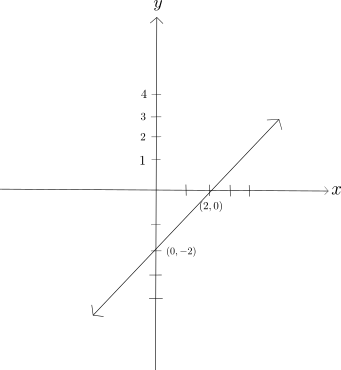
\includegraphics[width=7cm]{figures/problem7part1.png}
                    \label{fig:my_label}
                \end{figure}
            \end{solution}
        \item[(ii)] Let \( a,c \in \R  \) and \( b \in \C  \) with \( \overline{b}b - ac > 0  \) and
            \[  \zeta = \{  z \in \C : a | z |^{2} + \overline{b}z + b \overline{z} + c = 0 \}.  \]
            \begin{solution}
            Let \( z = x + iy \) and \( b = u + iw \) for \( x,y,u,w \in \R  \). Then observe that 
            \begin{align*}
                0  = a | z  |^{2} + \overline{b}z + b \overline{z} + c &= a (x^{2} + y^{2}) + (u-iw)(x+iy) + c  \\
                                                                 &= ax^{2} + ay^{2} + 2ux + 2wy + c 
            \end{align*}
            which imply that 
            \begin{align*}  
                \Big[ x^{2} + \frac{ 2ux }{ a }  + \Big( \frac{ u }{ a }  \Big)^{2} \Big] +  \Big[ y^{2} + \frac{ 2wy }{ a }  + \Big(  \frac{ w }{ a }  \Big)^{2} \Big]  &= \frac{ u^{2} + w^{2} - ac  }{ a }
                                                             \end{align*}
            which further implies that 
            \[   
                \Big(  x^{2} + \frac{ u }{ a }  \Big)^{2} + \Big( y^{2} - \frac{ w }{ a }  \Big)^{2}                                                                                                                                                          = \frac{ | b |^{2} - ac  }{ a }. 
            \]
            Set 
            \[  \gamma = \frac{ | b |^{2} - ac  }{ a  }  \]
            and so
            \[  \frac{ \Big(  x^{2} + \frac{ u }{ a }  \Big)^{2} }{ \gamma  } + \frac{ \Big( y^{2} - \frac{ w }{ a }  \Big)^{2} }{ \gamma  }  = 1 \]
            which is an equation of a circle with radius \( \gamma > 0 \).
                \begin{figure}[H]
                    \centering
                    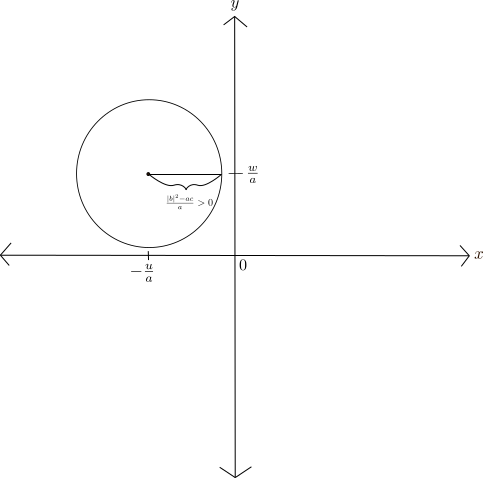
\includegraphics[width=7cm]{figures/problem7part2.png}
                    \label{fig:my_label}
                \end{figure}

            \end{solution}
        \item[(iii)] \( \zeta = \{ z \in \C : | z - i  |  = 2  \}  \).
            \begin{proof}
            Let \( z = x + iy  \) for \( x,y \in \R  \). Then we see that 
            \begin{align*}
                | z - i  |^{2} = 4 &\implies (z - i) \overline{(z - i)} = 4 \\
                                   &\implies (x + i(y-1))(x - i(y-1)) = 4 \\
                                   &\implies x^{2} + (y-1)^{2} = 4 \\
                                   &\implies \frac{ x^{2} }{ 4 } + \frac{ (y-1)^{2} }{ 4 }  = 1
            \end{align*}
            which is an equation for a circle in \( \R^{2} \). Thus, we have
                \begin{figure}[H]
                    \centering
                    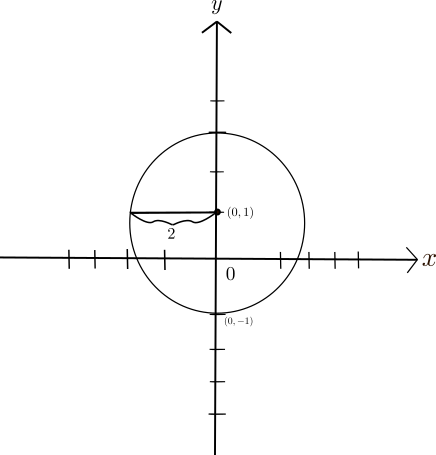
\includegraphics[width=7cm]{figures/problem7part3.png}
                    \label{fig:my_label}
                \end{figure}
            \end{proof}
    \end{enumerate}


    \section*{Problem 8} Let \( z,a \in \C  \). 
        \begin{enumerate}
            \item[(i)] Show that \( |  1 - z \overline{a} |^{2} - | z - a  |^{2} = (1 - | z | )^{2} (1 - | a |^{2}) \).
                \begin{proof}
                Note that \( | a  |^{2} = | \overline{a} |^{2}  \) and that  
                \[ \langle z  , a  \rangle = \Re(z \overline{a}) = x u + yv =   \Re(\overline{z} a ) = \langle 1  ,  z \overline{a} \rangle. \]
                if \( z = z + iy \) and \( a = u + iv  \) for \( x,y,u,v \in \R  \).
                Observe that 
                \begin{align*}
                    |  1 - z \overline{a} |^{2} - | z - a  |^{2} &= [ 1 - 2 \langle 1  , z \overline{a} \rangle + | z \overline{a} |^{2}] - [ | z  |^{2} - 2 \langle z , a \rangle + | a |^{2}] \\
                                                                 &=  | z  |^{2} | a |^{2} - | z |^{2} - | a |^{2} - 1  \\ 
                                                                 &= (1 - | z |^{2})(1 - | a |^{2}).
                \end{align*}
                Hence, we see that 
                \[  |  1 - z \overline{a} |^{2} - | z - a  |^{2} = (1 - | z |^{2})(1 - | a |^{2}). \]
                \end{proof}
            \item[(ii)] Assume that \( | a  |  < 1  \). Show that 
                \[  | z  |  < 1 \iff \Big| \frac{ z - a  }{ 1 - \overline{a} z  } \Big| < 1     \tag{1}\]
                and
                \[  | z  |  = 1 \iff \Big| \frac{ z - a  }{  1 - \overline{a} z  }  \Big|  = 1. \tag{2} \]
                \begin{proof}
                Suppose \( |  z  | < 1  \) and \( | a  |  < 1  \). We will first show that  the forwards direction of (1).
                \[  \Big|  \frac{  z - a  }{ 1 - \overline{a} z  }  \Big| < 1.  \]
                It suffices to show that 
                \[  | z - a  |^{2} < | 1 - \overline{a}z |^{2}.  \]
                By part (i), we see that 
                \[  | z - a  |^{2} = | 1 - z \overline{a} |^{2} - (1 - | z |^{2})(1 - | a |^{2}). \tag{3}\]
                Since \( | z  |  < 1  \) and \( | a  |  < 1  \), we see that 
                \begin{center}
                    \( 1 - | z  |^{2} > 0  \) and \( 1 - | a |^{2} > 0 \). 
                \end{center}
                Thus, we see that 
                \[  -(1-| z |^{2} )(1 - | a |^{2}) < 0. \]
                Therefore, (3) implies that 
                \[  | z - a  |^{2} < | 1 - \overline{a}z  |^{2} \]
                which further implies that 
                \[  \Big| \frac{ z - a  }{ 1 - \overline{a}z }  \Big| < 1. \]

                Now, suppose for the backwards direction that 
                \[  \Big| \frac{  z - a  }{  1 - \overline{a}z }  \Big|  < 1. \]
                Note that this is equivalent to saying
                \[  | z - a  |^{2}  < | 1 - \overline{a }z  |^{2}  \]
                By using the fact that 
                \[  | z - a  |^{2} = | z  |^{2} - 2 \langle z  , a \rangle + | w  |^{2} \]
                and 
                \[  | 1 - \overline{a}z |^{2} = 1 - 2 \langle 1  , \overline{a} z  \rangle + | \overline{a}z  |^{2}.  \]
                Then observe that 
                \begin{align*}
                    | z - a  |^{2} < | 1 - \overline{a}z |^{2} &\implies   
                    | z  |^{2} - 2 \langle z , a \rangle + | w  |^{2} < 1 - 2 \langle 1  , \overline{a}z \rangle + | \overline{a} |^{2} | z  |^{2}.
                \end{align*}
                So, we must have 
                \begin{align*}
                    | z  |^{2} - 2 \langle z , a \rangle + | a |^{2} &< 1 - 2 \langle 1  , \overline{a}z \rangle + | \overline{a} |^{2} | z |^{2} \\
                    | z |^{2} + | a |^{2} &< 1 + | a |^{2} | z |^{2} 
                \end{align*}
                which imply that 
                \begin{align*}
                    | z |^{2} < ( 1 - | a |^{2}) + | a |^{2} | z |^{2} &\implies | z  |^{2} ( 1 - | a |^{2} ) < 1 - | a |^{2}   \\
                                                                       &\implies | z  |^{2}  < \frac{ 1 - | a |^{2}  }{  1 - | a |^{2}  }  = 1.
                \end{align*}
                Thus, we see that \( | z  | < 1  \). To prove (2), we can replace the inequalities above with an equal sign and the proof will be the same.
            \end{proof}
        \end{enumerate}


\end{document}
